\chapter{\protect\textsc{Carico}}
% This chapter may be called something else\ldots but in general the
% idea is that you have one (or a few) ``meat'' chapters which describe
% the work you did in technical detail.
% \begin{tcolorbox}[boxsep=0mm,left=2.5mm,right=2.5mm]
    % \textbf{Design and Implementation:} {\em In this section, I will outline the
    % goals of my system. I will give a brief overview of the chapter structure,
    % summarising each core section and what I achieve.}
% \end{tcolorbox}
This chapter details \textsc{Carico}, a federated, asynchronous,
memory-limited algorithm, building upon the principles of \textsc{Pronto}.
\textsc{Carico} differentiates itself from \textsc{Pronto} for the following
reasons:
\begin{enumerate}
    \item Rather than performing standard FPCA, \textsc{Carico} applies FSVD on
        non-centered observed resource usage. Subsequently, \textsc{Carico} uses
        new interpretations for the results of SVD and presents a modification
        of the Subspace-Merge to preserve the interpretations.
    \item \textsc{Carico} presents a novel continuous and \textbf{comparable}
        capacity signal function that combines the new model interpretations
        with a Node's current resource usage to calculate the estimated workload
        capacity.
    \item \textsc{Carico} makes two assumptions to translate the calculated
        capacity signal into a signal that is both \textbf{reservable} and uses
        the number of Pods as its unit of measure.
\end{enumerate}
As this algorithm produces a signal that measures "capacity", I will refer to it
as \textsc{Carico} - "load" in Italian.

\section{Capacity Signal}
In Section \ref{sec:intro-weakness}, we identified critical limitations of
\textsc{Pronto}'s binary ``Reject-Job" signal within the Kubernetes ecosystem:
its lack of comparable Node scoring and inability to handle Pod startup
latencies. While one could conceivably compare the number of detected spikes,
this does not translate into a reservable signal, meaning it's impossible to
quantitatively assign or reserve ``peak detections" for incoming Pods.
Furthermore, as empirically demonstrated in Figure
\ref{fig:podcount-util-pressure}, contention metrics often do not change
proportionally to the number of tasks assigned, making them difficult to reserve
accurately.

To overcome these limitations, a signal reflecting varying levels of contention
and offering a predictable, scalar relationship with task assignments was
necessary. This led us to reconsider a metric of capacity. Supported by its use
within \texttt{kube-scheduler}, this approach provides the necessary properties
to make it compatible with reservation mechanisms. To produce a measure of
capacity, we had to deviate from FPCA as its interpretations focused on the
variability within telemetry data rather than its magnitude. The subsequent
challenge was to find a means of transforming \textsc{Pronto}'s mathematical
framework to produce values that could be interpreted as the direction and
magnitude of recent workload's resource usage. Only once we had this
interpretation, could we then develop a continuous, comparable, and reservable
signal that could effectively and accurately guide scheduling decisions.

\section{Local Model}
\label{sec:local-model-construction}
\textsc{Pronto} has each individual compute node build a local model of its
resource usage by performing iterative-SVD on incoming batches of
mean-centered telemetry data and its latest local model. The resulting
$\mathbf{U}$ can be interpreted as the PCs of the original telemetric data, and
the singular values in $\Sigma$ can be used to weight the different PC
projections accordingly.

\textsc{Carico} assumes that the telemetric data collected by Nodes is
[0,1]-normalised. A batch of telemetric data $\mathbf{A}$ is an $m \times n$
matrix, where $\mathbf{A}$ contains $n$ samples of $m$-dimensional columns of
data. Each dimension in the vector represents a different resource, where the
value $0$ indicates that full capacity is available for that resource and $1$
indicates that the resource is being fully used. This means results in
$\mathbf{A}$ being non-negative with $0 \leq a_{ij} \leq 1$ for all $i,j$. As we
are no longer mean-centering the dataset before applying SVD, \textbf{PCA's
interpretations no longer apply to the resulting $\mathbf{U}$ and $\Sigma$
matrices}.

Instead, \textsc{Carico} is built on top of  a different set of interpretations.
Using the Lemma proved in Appendix \ref{app:vector-to-avg}, we can interpret the
first left singular value $u_1$ in $\mathbf{U}$ as a pseudo-weighted average
direction of the datapoints in the matrix: ``larger" or more aligned columns
contribute more significantly to the sum defining $u_1$, and thus to its final
direction. \textsc{Carico}, thus uses $u_1$ as a primary indicator of the
direction of the current workload's resource usage.

While knowing the proportion of resource usage is useful, it is also important
to be able to differentiate between lightweight workloads and more intense
workloads. For this, \textsc{Carico} uses the first singular value $\sigma_1$ in
$\Sigma$. Given $\sigma_1(\mathbf{M})$ and $u_1$ correspond to the first singular value and
first left singular vector of the non-negative matrix $\mathbf{M}$, the
following holds:
\begin{align}
    \sigma_1(\mathbf{M})^2 &= u_1^T \mathbf{MM}^T u_1 \\
    &= (u_1^T \mathbf{M})^2
\end{align}
Given $m_j$ is the $j$-th column of $\mathbf{M}$, $\sigma_1(\mathbf{M})^2$ can be
interpreted as the sum of squared scalar projections of columns in $\mathbf{M}$:
$\sigma_1(\mathbf{M})^2 = \sum_{j=1}^n (u^T m_j)^2$.

Furthermore, the first singular value can be shown to scale with resource usage.
Given two batches of telemetry $\mathbf{A}$ and $\mathbf{B}$ where batch
$\mathbf{B}$ experienced more resource usage ($0 \leq a_{ij} \leq b_{ij} \leq 1$
for all $i,j$), it is shown in Appendix \ref{sec:app-monotonicity} that the
first singular value of $\mathbf{B}$ will be greater than or equal to that of
$\mathbf{A}$ ($\sigma_1(\mathbf{A}) \leq \sigma_1(\mathbf{B})$. With these
properties, the first singular value makes a good indicator of measured resource
usage.

\section{Subspace Merging}
\label{sec:local-merge}
While we have shown that the results from performing SVD on [0,1]-normalised
telemetry data can have useful interpretations, the resulting $\sigma_1$ can
grow with each iterative-SVD:\\
Given two non-negative matrices $\mathbf{A} \in \mathbb{R}^{m \times n_1}$ and
$\mathbf{B} \in \mathbb{R}^{m \times n_2}$, the first singular value of the
concatenated matrix $\mathbf{C} = [\mathbf{A}, \mathbf{B}]$ is greater than or
equal to the maximum of the first singular values of $\mathbf{A}$ and
$\mathbf{B}$. That is,
\[ \sigma_1([\mathbf{A}, \mathbf{B}]) \geq \max(\sigma_1(\mathbf{A}),
\sigma_1(\mathbf{B})) \]
This is proved in Appendix \ref{sec:app-concatenate}.

This property is important, as we established earlier that $\sigma_1$ is used by
\textsc{Carico} as an indicator of the magnitude of resource usage. If
$\sigma_1$ can increase while the measured telemetry reports a stable magnitude
of resource usage, its interpretation no longer holds.

A solution is to scale the concatenated matrices using non-negative scalar
weights $\gamma_{\mathbf{A}} = \sqrt{w_{\mathbf{A}}}$ and
$\gamma_{\mathbf{\mathbf{B}}} = \sqrt{w_{\mathbf{\mathbf{B}}}}$ such that
$w_{\mathbf{A}} + w_{\mathbf{\mathbf{B}}} = 1$. This method still preserves the
earlier interpretations:

\begin{itemize}
    \item \textbf{First Left Singular Vector:}\\
        The resulting first singular vector $u_1$ of the concatenated matrix $\mathbf{C} =
        [\gamma_{\mathbf{A}}\mathbf{A},
        \gamma_{\mathbf{\mathbf{B}}}\mathbf{\mathbf{B}}]$ still behaves as a
        pseudo-weighted average, but with the contributions of the input telemetry
        further weighted according to the scalar weights. This is useful as using
        different values for $\gamma_{\mathbf{A}}$ and $\gamma_{\mathbf{B}}$ behaves
        similarly as the forget factor $\gamma$ used in \textsc{Pronto}.
    \item \textbf{First Singular Value:}\\
        In addition, Appendix \ref{sec:app-scale} proves that the resulting first
        singular value and the first left singular vector of the concatenated matrix
        $\mathbf{C} = [\gamma_{\mathbf{A}}\mathbf{A},
        \gamma_{\mathbf{B}}\mathbf{B}]$ has the following property:
        \[ \min(P_{\mathbf{A}}(u_{\mathbf{C}}),P_{\mathbf{B}}(u_{\mathbf{C}}))
        \leq \sigma_1(\mathbf{C})^2 \leq
        \max(P_{\mathbf{A}}(u_{\mathbf{C}}),P_{\mathbf{B}}(u_{\mathbf{C}})) \]
        where $\sigma_{\mathbf{C}}$ and $u_{\mathbf{C}}$ correspond to the first
        singular value and first left singular vector of $\mathbf{C}$,
        $P_{\mathbf{M}}(u)$ is the sum of squared scalar projections of the
        columns in $\mathbf{M}$ onto $u$ (let $m_j$ be the $j$-th column of
        $\mathbf{M}$ $P_{\mathbf{M}}(u) = \sum_{j=1}^n (u^T m_j)^2$). As
        $\sigma_1(\mathbf{C})^2$ is a convex combination of
        $P_{\mathbf{A}}(u_{\mathbf{C}})$ and $P_{\mathbf{B}}(u_{\mathbf{C}})$,
        it is effectively a weighted mean of these two projected sums and
        ensures $\sigma_1$ grows with the magnitude of the observed resource
        usage.
\end{itemize}

\section{Capacity Signal Function}
\label{sec:capacity-signal}
Using the interpretations established above:
\begin{itemize}
    \item $u_1$: the pseudo-weighted average direction of resource usage of
        recent workloads
    \item $\sigma_1$: the magnitude of the resource usage of recent workloads
\end{itemize}
we can calculate a new capacity signal that considers both the estimated
workload resource usage and its current resource usage. Given the the current
[0,1]-normalised resource usage vector for the node $y$, the first singular
value and left singular vector $\sigma_1$, $u_1$ from the latest $U$ and
$\Sigma$, a Node's estimated capacity signal $k$ is given by:
\begin{align}
    y_{\text{predict}} = y + k * \sigma_1 u_1 \\
    \max_k \forall i: y_{\text{predict}} < 1
\end{align}
The resulting $k$ represents how many "units" of the learned ``average" workload
($\sigma_1 u_1$) can be added to the current workload ($y$) before any single
resource dimension hits its normalised capacity of 1. In the following sections,
I will refer to $k$ as ``Capacity".

% This calculation does
% ignore the fact that $\sigma_i^2$ is a sum of $n$ projected distances, where $n$
% is the number of samples. However, this will only matter if compute nodes use
% different batch sizes, otherwise, this $\frac{1}{\sqrt{n}}$ factor is absorbed
% into $k$.
%
\subsection{Example Scenarios}
\label{sec:signal-example-scenario}
To better understand how this signal works, I will explore how the signal
changes under different different loads. This scenarios will also be used to
control the correctness of the signal implementation in the prototype.

\begin{figure}[ht]
    \centering
    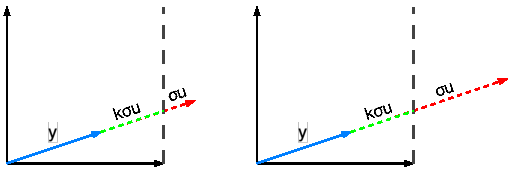
\includegraphics[width=\textwidth]{images/conflicting-workload.pdf}
    \caption{Visualisations of a Node's resource usage $y$ and expected resource
    usage $\sigma_1 u_1$ when learning of conflicting resource utilisation.}
    \label{fig:conflicting-workload}
\end{figure}

Figure \ref{fig:conflicting-workload} presents the scenario where a Node updates
its local model, learning that the experienced workload has increased in
resource usage ($\sigma_1$ has increased). This means that a smaller constant
$k$ is needed before the combined vectors cross a resource boundary. As a
result, a Node advertises a smaller capacity signal as it has less capacity for
the expected resource usage.

\begin{figure}[ht]
    \centering
    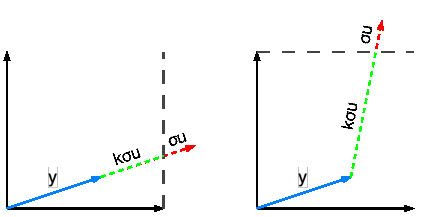
\includegraphics[width=0.8\textwidth]{images/complementary-workload.pdf}
    \caption{Visualisations of a Node's resource usage $y$ and expected resource
    usage $\sigma_1 u_1$ when learning of complementary resource utilisation.}
    \label{fig:complementary-workload}
\end{figure}

Figure \ref{fig:complementary-workload} presents the scenario where a Node updates
its local model, learning that the learned workload is using more resources but
in a different direction. This could be described as a complementary workload as
the the dot product of the current resource utilisation and the expected
resource utilisation is much smaller. Therefore, a larger constant $k$ is needed
to cross a resource boundary. This results in a Node advertising a higher
capacity signal as it has more capacity for the new expected resource
utilisation.

\section{Reserve Cost and Capacity}
\label{sec:spazio-cost-capacity}
Like \textsc{Pronto}, \textsc{Carico}'s signal uses its current resource usage, and therefore, only
reflects Pods that have been scheduled and are running on the Node. For \textsc{Carico}
to work in a system with Pod startup latency, the scheduler must be able to
predict the effect a Pod will have on a Node's signal. \textsc{Carico} assumes that Nodes
know the number of currently running Pods, as well as, have the ability to
estimate their:
\begin{enumerate}
    \item \textbf{Baseline Capacity Signal:} the Capacity signal when no Pods
        are running
    \item \textbf{Per-Pod-Cost:} the estimated amount that the Capacity signal
        will drop when a single Pod starts running.
\end{enumerate}
Section \ref{sec:estimating-cost} implements and compares different prediction
methods. With this information, a Node can calculate its Pod-Capacity from:
\begin{align}
    \text{Pod-Capacity} &= \frac{\text{Current Capacity Signal}}{\text{Per-Pod-Cost}} \\
    \text{Pod-Capacity} &= \frac{\text{Baseline Capacity Signal}}{\text{Per-Pod-Cost}}
    - \text{Current Pod Count}
\end{align}
This metric has two useful properties:
\begin{itemize}
    \item \textbf{Dual-Mode:} Pod-Capacity can be calculated
        using two equations. This is especially useful in Kubernetes as during
        the creation or deletion of a Pod, the measured resource usage
        can experience large spikes. While filtering can mitigate these spikes,
        they are still observable in Figure \ref{fig:filtered-metrics-eval}. To
        combat this noise, Nodes can switch to predicting Pod-Capacity using
        estimated capacity and Pod count. This reduces fluctuations in a Node's
        advertised capacity and improves scheduling decisions
    \item \textbf{Unit of Measure:} Pod-Capacity's  unit of measure is in terms
        the number of Pods. This simplifies the central scheduler's logic as it
        does not need to keep track of each Node's Per-Pod-Cost.
\end{itemize}

Each Node $n$ will broadcast its $\text{Pod-Capacity}_n$ to a central scheduler. This
scheduler also tracks each Node's reserved amount as $\text{\# Pods Reserved}_n$. For
each Pod waiting to be assigned to a Node, the scheduler performs the following
operations:
\begin{itemize}
    \item \textbf{Filter:} Filters out all Nodes $n$ with $\text{Pod-Capacity}_n -
        \text{\# Pods Reserved}_n < 1$. Ensures we do not schedule on Nodes that do not
        have enough resources for another pod. While we could reduce the limit
        to improve throughput by packing more Pods on a Node, it could result in
        OOM kills if there isn't enough memory available on a Node for all of
        the Pods.
    \item \textbf{Score:} Score Nodes $n$ by $\text{Pod-Capacity}_n - \text{\#
        Pods Reserved}_n$. This ensures we allocate to Nodes which can fit more
        Pods.
    \item \textbf{Reserve:} Once a node is Node has been chosen, we increment
        $\text{\# Pods Reserved}_n$ by $1$ for that Node. Once a scheduled Pod
        is no no longer in the Pending state, the central scheduler decrements
        $\text{\# Pods Reserved}_n$ by $1$ for the Node $n$ the Pod was assigned
        to.
\end{itemize}

\section{Properties}
\textsc{Pronto} is designed to be \textit{federated, streaming} and
\textit{unsupervised}. \textsc{Carico} exhibits identical properties while also
considering the existance of communication and Pod startup latency.

\textbf{Federated:} \textsc{Pronto} executes scheduling plans in a decentralised fashion
without knowledge of the global performance dataset. Such approach in
Kubernetes could actually decrease performance. The Kubernetes API server
handles the publishing and updating of Kubernetes objects. A decentralised
system with no global synchronisation or coordination could result in a
stampede of Bind requests that could overload the Kubernetes API server and slow
down the publishing of incoming Pods. Instead, \textsc{Carico} uses a central scheduler
to score Nodes and perform the final Bind operation. However, it can still be
considered federated because of its use of federated SVD \cite{}: individual
Nodes can have a unified view of the global workload while maintaining their
individual autonomy to set their score as they deem fit.

\textbf{Streaming:} \textsc{Carico}'s use of iterative-SVD, like \textsc{Pronto}, means it only
requires memory linear to the number of features considered; the required memory
is proportional to $\mathcal{O}(d)$. Furthermore, like \textsc{Pronto}, \textsc{Carico} only
requires a single pass over the incoming data without having to store historical
data in order to update its estimates.

\textbf{Unsupervised:} \textsc{Carico} uses FSVD and assumptions about the
collected telemetry to generate values with capacity-based interpretations.
While this greatly differs from \textsc{Pronto} and its use of FPCA,
\textsc{Carico} still exploits the resulting subspace estimate along with the
incoming data to reveal patterns in recent resource-usage.

\textbf{Continuous Value} \textsc{Pronto} is a binary signal, which makes difficult to
score Nodes. \textsc{Carico}'s $\text{Pod-Capacity} \in \mathbb{R}$, allowing
Nodes to be filtered and scored against each other.

\textbf{Latency Resilient:} Unlike \textsc{Pronto} which assumes no communication
latency, \textsc{Carico} was designed with Kubernetes in mind, and thus must consider
possible latency in communication and Pod startup. \textsc{Carico}'s
$\text{Pod-Capacity}$'s unit of measure allows the central scheduler to easily
track the estimated cost of Pods in-flight, ensuring subsequent scheduling
decisions do not mistakenly overload a Node with a high $\text{Pod-Capacity}$.
%
% There are several methods to integrating the reserve cost into the signal to be
% sent to the central scheduler. The first method involves sending the signal and
% the reserve cost as separate values. On pod bind, we reserve the latest pod cost
% from the signal, and only relinquish the reserved amount once the central
% scheduler \verb|kube-apiserver| listener detects the pod is no longer Pending.
% This method requires the central scheduler to keep track of both the pods on
% each node and the pod-cost when the pod was bound.
%
% I instead chose to integrate the reserve quantity directly into the signal: each
% node calculates its available capacity in terms of no. of pods using two equations:
% \[ \text{avail. capacity from signal} = \frac{\text{signal}}{\text{per-pod-cost}} \\
   % \text{avail. capacity from no. of pods} = \frac{\text{capacity}}{\text{per-pod-cost}} -
   % \text{no. of pods} \]
%
% We use to functions for different situations. Typically, we calculate the
% available capacity from the latest signal measurements. However, if we detect a
% recent container event, the remote \verb|pronto| pod calculates the capacity
% from the pod count. This is to reduce the instability introduced by the
% container runtime. Furthermore, with this signal, the central scheduler does not
% have to record the per-pod-cost at bind time as the signal is now given in terms
% of individual pod counts. This simplifies the central scheduler and reduces the
% memory demand on.
%
